\documentclass[../lecture-notes.tex]{subfiles}

\begin{document}

\subsection{Commitments}

\begin{definition}
    A cryptographic commitment scheme allows one party to commit to a chosen statement (such as a value, vector, or polynomial) without revealing the statement itself. The commitment can be revealed in full or in part at a later time, ensuring the integrity and secrecy of the original statement until the moment of disclosure.
\end{definition}

Imagine putting a letter into a box and locking it with your key. 
You then give that box to your friend, who cannot open it without the key.
In this scenario, you have made a commitment to the letter inside the box. 
You cannot change the content of the letter, as it is in your friend's possession. 
At the same time, your friend cannot access the letter since they do not have the key to unlock the box.

\begin{center}
    \centering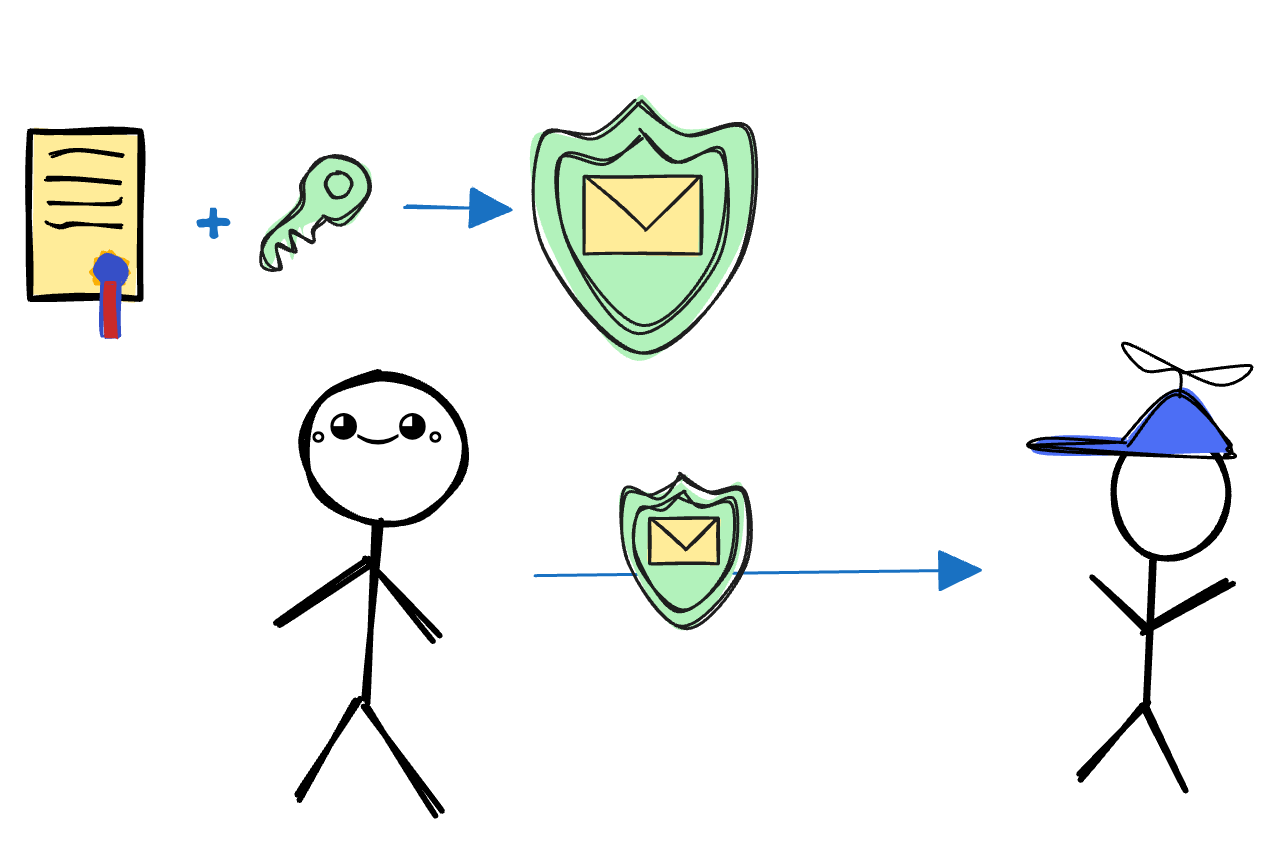
\includegraphics[width=0.5\linewidth, clip]{images/lecture_5/CommitmentExample.png}

    \scriptsize{\textbf{Illustration:} Commitment scheme}
\end{center}

\subsubsection{Hash-based commitments}

\end{document}